\documentclass{article}

% if you need to pass options to natbib, use, e.g.:
% \PassOptionsToPackage{numbers, compress}{natbib}
% before loading nips_2016
%
% to avoid loading the natbib package, add option nonatbib:
% \usepackage[nonatbib]{nips_2016}

\usepackage{nips_2016}

% to compile a camera-ready version, add the [final] option, e.g.:
% \usepackage[final]{nips_2016}

\usepackage[utf8]{inputenc} % allow utf-8 input
\usepackage[T1]{fontenc}    % use 8-bit T1 fonts
%\usepackage{hyperref}       % hyperlinks
\usepackage{url}            % simple URL typesetting
\usepackage{booktabs}       % professional-quality tables
\usepackage{amsfonts}       % blackboard math symbols
\usepackage{nicefrac}       % compact symbols for 1/2, etc.
\usepackage{microtype}      % microtypography
\usepackage{amsmath}
\usepackage{mathtools}
\usepackage{fancyvrb}
\usepackage{multirow}
\usepackage{color}

\usepackage{listings}
\definecolor{lightgray}{rgb}{.9,.9,.9}
\definecolor{darkgray}{rgb}{.4,.4,.4}
\definecolor{purple}{rgb}{0.65, 0.12, 0.82}
\definecolor{orange}{rgb}{1,0.5,0}

\definecolor{Red}{RGB}{255,0,0}
\newcommand{\red}[1]{\textcolor{Red}{#1}}
\definecolor{Green}{RGB}{10,200,100}
\definecolor{Blue}{RGB}{10,100,200}
\newcommand{\ndg}[1]{\textcolor{Green}{[ndg: #1]}}
\newcommand{\mht}[1]{\textcolor{Blue}{[mht: #1]}}
\newcommand{\lou}[1]{\textcolor{orange}{[lou: #1]}}

\lstdefinelanguage{JavaScript}{
  keywords={typeof, new, true, false, catch, function, return, null, catch, switch, var, if, in, while, do, else, case, break},
  keywordstyle=\color{blue}\bfseries,
  ndkeywords={class, export, boolean, throw, implements, import, this},
  ndkeywordstyle=\color{darkgray}\bfseries,
  identifierstyle=\color{black},
  sensitive=false,
  comment=[l]{//},
  morecomment=[s]{/*}{*/},
  commentstyle=\color{purple}\ttfamily,
  stringstyle=\color{red}\ttfamily,
  morestring=[b]',
  morestring=[b]"
}

\lstset{
   language=JavaScript,
   backgroundcolor=\color{white},
   extendedchars=true,
   basicstyle=\footnotesize\ttfamily,
   showstringspaces=false,
   showspaces=false,
   numbers=none,
   numberstyle=\footnotesize,
   numbersep=9pt,
   tabsize=2,
   breaklines=true,
   showtabs=false,
   captionpos=b
}



\usepackage[ruled,vlined]{algorithm2e}

\newcommand{\ud}{\,\mathrm{d}}
\newcommand{\argmax}{\operatornamewithlimits{argmax}}


\title{Practical optimal experiment design for psychology}

% The \author macro works with any number of authors. There are two
% commands used to separate the names and addresses of multiple
% authors: \And and \AND.
%
% Using \And between authors leaves it to LaTeX to determine where to
% break the lines. Using \AND forces a line break at that point. So,
% if LaTeX puts 3 of 4 authors names on the first line, and the last
% on the second line, try using \AND instead of \And before the third
% author name.

\author{
  David S.~Hippocampus\thanks{Use footnote for providing further
    information about author (webpage, alternative
    address)---\emph{not} for acknowledging funding agencies.} \\
  Department of Computer Science\\
  Cranberry-Lemon University\\
  Pittsburgh, PA 15213 \\
  \texttt{hippo@cs.cranberry-lemon.edu} \\
  %% examples of more authors
  %% \And
  %% Coauthor \\
  %% Affiliation \\
  %% Address \\
  %% \texttt{email} \\
  %% \AND
  %% Coauthor \\
  %% Affiliation \\
  %% Address \\
  %% \texttt{email} \\
  %% \And
  %% Coauthor \\
  %% Affiliation \\
  %% Address \\
  %% \texttt{email} \\
  %% \And
  %% Coauthor \\
  %% Affiliation \\
  %% Address \\
  %% \texttt{email} \\
}

\begin{document}
% \nipsfinalcopy is no longer used

\maketitle

\begin{abstract}
  The abstract paragraph should be indented \nicefrac{1}{2}~inch
  (3~picas) on both the left- and right-hand margins. Use 10~point
  type, with a vertical spacing (leading) of 11~points.  The word
  \textbf{Abstract} must be centered, bold, and in point size 12. Two
  line spaces precede the abstract. The abstract must be limited to
  one paragraph.
\end{abstract}

\section{Introduction}
\ndg{Doing the standard, active learning thing with probabilistic programs. }

Designing scientific experiments is hard.
Scientists must have hypotheses and reason over a potentially large space of possible experiments.
Studying human behavior has additional complications.
Human data is noisy and sensitive to dependent measure of the task. 
Further, human data is expensive and one must balance expected statistical power with the constraints of a limited budget to decide on the number of participants to run.

Formal models of psychological phenomena alleviate some of these issues.
Models are used to make explicit hypotheses about observed data, and thus make it easier (or in some cases, possible) to explore the implications of a set of ideas.
Exploring models is time-consuming however, and searching through a large space of possible experiments is still largely driven by the scientist's intuition and folk theory.
This need not be the case: If both the set of hypotheses and the space of experiments are stipulated explicitly, then \red{computation can drive experiment design}. \mht{<--replace computation with active learning; or otherwise, make less vague?}

We present a general, principled, and turnkey approach to designing experiments that uses Bayesian computation to find experiments that
best disambiguate competing hypotheses.
The framework is implemented in a \emph{probabilisitic programming language} (PPL). 
PPLs are a convenient way to represent explicit hypotheses about the data. 
We make it so the same language can be used to formalize hypotheses as well as run optimal experiment design (OED). 
This is a crucial step in making a practical OED system.

%Though the framework is Bayesian, it is not directly related to Bayesian models of cognition; rather, it can be applied to any instance in which the scientist has a formal model of the data generating process (including, Bayesian models of cognition).

We are not the first to attempt to develop a framework for optimal experiments in psychology. 
Previous attempts, however, suffer from a number of pragmatic issues that impede the scientist who wishes to readily apply OED to their research.
These include ad-hoc optimization criteria, a lack of established pipeline, 
and a lack of analysis in dealing with practical experimental concerns specific to psychology, including dealing with noisy responses from participants, determining ideal numbers of participants, and deciding upon appropriate dependent measures or linking functions.
Taken together, these issues put the burden on researchers to have sufficient expertise to adapt the OED system to their specific problem and
require researchers to develop their own system for writing formal psychological models and the OED optimization engine.

In this paper, we resolve these issues using a principled and general Bayesian model selection framework implemented in a practical modeling system.
We apply this framework to two case studies: the psychology of subjective randomness and categorization.
The first case study highlights the details of application for a simple space of experiments.
The second study applies OED to a more realistic space of possible experiments and validates our theoretical analysis by running the optimal experiment.
Our general system opens a number of rich areas for future development, which we discuss briefly at the end.

%We conclude by highlighting the generality of the approach and areas of future work.
%\ndg{all the parts are here. needs smoothing. make it clearer that using PPL to represent hypotheses is a key step in making the system practical.}

%    \begin{itemize}
%        \item It is difficult to discriminate models of psychological processes
%        \item Experiments are expensive
%        \item We present a general, turn-key approach to design experiments that best disambiguate competing models using a Bayesian framework
%        \item This technique is not directly related to Bayesian models of cognition. It can be used on any (formal / probabilistic) model, including Bayesian models of cognition
%        \item Despite the previous attempts in this field, there are a number of pragmatic issues that make it difficult to readily apply OED techniques for psychology, including:
%        \begin{itemize}
%            \item A variety of proposed optimization criteria, which puts the burden on researchers to have sufficient expertise to select the appropriate approach
%            \item A lack of an established pipeline, requiring researchers to develop a language to formalize psychological models and write an OED optimization engine
%            \item A lack of analysis in dealing with practical experimental concerns such as:
%                \begin{itemize}
%                    \item Noisy responses from participants
%                    \item The ideal number of participants for a study
%                    \item The ambiguity of linking functions of dependent measures
%                \end{itemize}
%        \end{itemize}
%    \end{itemize}


\section{Bayesian model selection framework}
\label{s:bayes}

\ndg{add a high-level overview of the setup first. describe the most general formulation (cognitive model of responses) and the more parsimonious bayesian modeling version where the response distribution is factored into belief-update cognitive models and a linking functions per DM that are shared across models.  point out some of the typical expt design knobs, such as number of Ss (relation to power analysis), dependent measures, etc. An overview schematic of the system could be useful?}

\ndg{after this overview, the remainder of this section can be streamlined a lot for NIPS.}

Psychological hypotheses can be expressed as computational models which make quantitative predictions about participants' responses. 
The Bayesian cognitive modeling framework factors out the \emph{cognitive}, or belief-updating, component from the mapping from latent beliefs to observed responses (so-called \emph{linking function}).
The cognitive model expresses the hypothesis, and the scientific community is often interested in which cognitive model (i.e. which hypothesis) best explains ``the data''.
``The data'', however, is a function of what experiments you chose to run, and experiment design is the process of deciding upon a subset of experiments (and the associated details of experiments) from a space of possible experiments. 
We introduce a framework which maps experiments to their expected information gain, with the goal being to disambiguate alternative cognitive models. 

For a set of possible experiments, $\mathcal{X}$, let the choice of experiment be defined as $x \in \mathcal{X}$.\footnote{
The most general notion of an ``experiment'' includes different design considerations such as the experimental prompt or item, the number of participants and the dependent measure of the task.  For the derivation, we consider all of these as part of the ``experiment''. \mht{<-- not sure this is right.}
} 
Similarly, for a set of possible responses, $\mathcal{Y}$, let $Y_x \in \mathcal{Y}$ be defined as a random variable that describes the distribution over the possible responses to the experiment $x$. 
Finally, for a set of candidate models, $\mathcal{M}$, let $M \in \mathcal{M}$ be a random variable that describes the uncertainty over which model best represents the underlying phenomenon of interest. 
\mht{ Is it confusing that  $\mathcal{M}$ is the set of candidate models, but $M \in \mathcal{M}$ is not a model?}
A model $m$ defines a stochastic relationship between the experimental setup and responses.
For a given model $m$, let the probability of observing a response $y$ given an experiment $x$ be defined as $x \rightarrow Y_{x,m}: P(Y_{x,m} = y_{x,m} | M = m)$.\footnote{
We use upper case symbols to represent random variables and lower case symbols to represent their corresponding realizations. For brevity, the probability of observing a particular realization will often be written without the random variable and using only the lower case symbol -- $p(y_{x,m} |m)$ represents $P(Y_{x,m} = y_{x,m} | M = m)$.
}
\ndg{should we have model explicit in this notation: $Y_{x,m}$?} \mht{I think so. Does the little $y$ take the subscript too?}

The goal of OED is to reason over the uncertainty $M$ of which model $m$ best represents the underlying phenomenon of interest. We quantify this uncertainty as a \emph{prior model belief distribution}, $p(m)$: It expresses the uncertainty before any experimental data is observed. 
%The choice of this distribution is a design decision by the experimenter. Often, uninformative priors, such as assuming that all candidate models are equally plausible, are good starting points. However, informative priors, which favor a particular subset of models \emph{a priori}, can be used when prior knowledge about the domain, such as previously collected data or established literature, is available.
The model belief distribution updates to a \emph{posterior model belief distribution} by observing a response. Using Bayes' theorem, the uncertainty of the model $m$ after observing the response $y_x$ is:
\begin{align}
p(m|y_x) = \frac{p(y_x|m)p(m)}{\sum\limits_{m'} p(y_x|m')p(m')}. \label{eq:bayes}
\end{align}
The posterior, $p(m|y_x)$, is solely a function of the model predictions, $p(y_x|m)$, and the prior, $p(m)$.

The \emph{efficacy} of an experiment is defined by its ability to differentiate between the candidate models, or equivalently, induce a change in our belief in the model. We quantify this change using the Kullback-Liebler divergence (KL divergence), a non-symmetric relative measure between two probability distributions, to compute the information gain between the posterior and prior distributions for a given experimental:
\begin{align}
D_{\text{KL}}\left(p(m|y_x) || p(m)\right) = \sum\limits_m p(m|y_x) \ln \left( \frac{p(m|y_x)}{p(m)}\right). \label{eq:kl}
\end{align}
This measure computes the amount of extra information required to encode the posterior distribution using the prior distribution. If the prior and posterior distributions of model beliefs are identical, then no additional information is required for the encoding and the information gain is zero, consistent with the intuition that an experiment that did not change our belief in the model was useless. As the posterior and prior diverge, then information gain increases and the associated experiment is better at differentiating between the candidate models.\footnote{For our framework, we use the natural logarithm, which corresponds to measuring information with the unit \emph{nats}.This choice was a matter of preference, and logarithms with different bases, such as 2 or 10, are also reasonable choices.}

So far, we've examined the information gain for a specific response, $y_x$.
Of course, human data is not deterministic; so, we must consider the whole data set.
The optimal experiment $x^*$ maximizes the expected KL divergence over the space of responses:

\begin{align}
x^{*} &= \argmax_{x} \sum\limits_{y_x} p(y_x) D_{\text{KL}}(p(m|y_x) || p(m)) \notag \\
    &= \argmax_{x} \sum\limits_{y_x} \left[\sum\limits_{m'} p(y_x|m')p(m')\right] D_{\text{KL}}(p(m|y_x) || p(m)). \label{eq:oed}
\end{align}

Since Eq.~\ref{eq:kl} measures the information gain for a single response, taking the expected value of the KL divergence obtains the average information gain weighted by the probability of observing a response. This measure, Eq.~\ref{eq:oed}, defines the OED criteria as a function of only the experimental condition. The probability of observing a result, $p(y_x)$, is computed by using its conditional probability, which leverages the model predictions, $p(y_x|m)$, and the prior, $p(m)$.
\footnote{It is worth noting that the expected KL divergence OED criteria, Eq.~\ref{eq:oed}, can be reformulated as the mutual information between the random variables for model belief, $M$, and response distribution, $Y_x$:
\begin{align}
x^* = \argmax_{x} \sum\limits_{y_x} p(y_x) D_{\text{KL}}(p(m|y_x) || p(m)) &= \argmax_{x} I(M, Y_x) \notag \\
    &= \argmax_{x} \sum\limits_{y_x} \sum\limits_{m} p(m, y_x) \ln \left( \frac{p(m, y_x)}{p(m)p(y_x)}\right). \label{eq:mi}
\end{align}
This reformulation uses a well-known identity between mutual information and the expected KL divergence~\cite{cover91:eit}. Mutual information is a measure of the amount of information one random variable contains about another, which provides an alternative perspective about the relationship between model belief and responses.
%This relationship, along with similar identities, will be useful for proving intrinsic properties about OED in Section~\ref{s:npart:ss:math}.
\ndg{if this doesn't get used in this version of the paper, then move to footnote?}
}
This OED framework is available as a package for the probabilisitic programming language WebPPL, and can be found at \url{https://github.com/mhtess/webppl-oed}

\section{Case study 1: Subjective randomness}
\label{s:tutorial}

We demonstrate the functionality of practical OED with a case study about subjective randomness. 
Human judgments about randomness are surprisingly systematic and nonuniform across equally random outcomes -- for example, a sequence of outcomes of coin flips \lstinline{HTHTTTHH} is considered to be more random than the sequence \lstinline{HHHHHHHH}. Of course, any sequence of coin flips is as equally likely than any other sequence, yet human intuitions strongly favor certain sequences when judging randomness ~\cite{goodfellow38:jep, griffiths01:cogsci}. 
%This discrepancy between human intuitions and statistical fact about randomness has garnered significant attention from both the mathematical~\cite{chaitin01:er, kac83:as, li97:kca} and psychological~\cite{falk81:pme, lopes82:jep, griffiths01:cogsci} literature.

There are several hypotheses one might have about what underlies human intuitions about randomness. Here, we consider two such hypothesis: (a) \emph{Weighted coin hypothesis}: Participants reason about the weight of the coin (i.e., the probability of a \lstinline{H} outcome), and (b) \emph{Markov coin hypothesis}: participants reason about the transition probabilities between \lstinline{H} and \lstinline{T} outcomes. 

%Consider two models of randomness judgements: independent flips from a biased coin and a sequence of flips from a Markov chain. These models are not supposed to fully characterize the neither intricacies of human judgments about randomness nor all hypotheses one could have about subjective randomness; rather, they provide a practical case study for understanding how optimal experiment design can be used to differentiate competing models.


%For now, we focus on the experimental prompt, and return to other design considerations in the Discussion.

 % Could be used in overview;;;;
%Before applying experiment design, one must define the experiment design space as well as the set of candidate models to be distinguished. The experiment design space characterizes the set of all design considerations that can be directly manipulated by the experimenter to generate distinct experimental conditions. Next, the experimenter must define a set of formal models that can predict the likelihood of observing a response for each experimental condition.

%This allows us to address experiment design concerns such as: ``which experimental prompt should I use?'', ``how many participants do I need?'', ``should I use a forced-choice dependent measure or a likert scale?''


%In this section, we describe the mathematical and theoretical framework of practical OED in detail. Although this section is intended to provide readers with a rigorous and formal foundation for understanding the principles behind our approach, an open source computational implementation is readily available for those who are interested in applying practical OED to their own models \red{(REF)}.
%This section provides a preliminary overview of the general mathematic concepts, with additional theoretical analysis in Sections~\ref{s:class:ss:math} and \ref{s:npart:ss:math}, which examines the role of model parameterization and the number of participants, respectively.


%\subsection{Models of subjective randomness}
%\label{s:tutorial:ss:randomness}

We consider the experimental scenario wherein participants will observed the outcomes of a coin being flipping four times and be prompted to predict whether the next flip will come up heads or tails. The space of subjective randomness models under consideration is $\mathcal{M} \in \{m_w, m_m\}$, where $m_w$ and $m_m$ correspond to the weighted coin model and the Markov coin model, respectively. 
The space of experimental prompts, $\mathcal{X}$, is the set of all sequences comprised of four flip coin flips, and the space of responses, $\mathcal{Y}$, is a choice between heads or tails.

\subsubsection{Weighted coin model}
\label{s:tutorial:sss:biased}

The weighted coin model assumes that the coin has some unknown bias and each coin flip is independent. 
The coin weight is inferred from the experiment prompt sequence (on a trial-by-trial basis), and it is subsequently used to predict the next coin flip. We show the model in the probabilistic programming language WebPPL \cite{dippl}.
%
\begin{lstlisting}[caption=Biased coin model]
var coin_weights = [0.01,0.1,0.2,0.3,0.4,0.5,0.6,0.7,0.8,0.9,0.99]

var weightedCoin = function(seq) {
  Enumerate(function(){
    var bias_p = uniformDraw(coin_weights);
    var logLkhd = binomialERP.score([bias_p,seq.length], sum(seq))
    factor(logLkhd)
    return flip(bias_p)
  })
}
\end{lstlisting}
%
The model first samples a coin weight \lstinline{bias_p} from a discretized uniform distribution over coin weights, and then computing the log-likelihood \lstinline{logLkhd} of the observed number of heads \lstinline{sum(seq)} given the weight \lstinline{bias_p} and the length of the sequence \lstinline{seq.length} (assuming a binomial likelihood). The model returns the posterior predictive distribution over the next outcome \lstinline{flip(bias_p)}.



\subsubsection{Markov coin model}
\label{s:tutorial:sss:markov}
The Markov coin model assumes that the coin is generated by a Markov process where each coin flip depends on the previous coin flip. The probability of transitioning from the current coin flip is inferred from the experiment prompt sequence (again, on a trial-by-trial basis), and is subsequently used to predict the next coin flip.
%
\begin{lstlisting}[caption=Markov coin model]
var markovCoin = function(seq) {
  Enumerate(function(){
    var transition_p =  uniformDraw(coin_weights);
    var logLkhd = sum(map2(function(x,y) {
    		var p = x ? 1-transition_p : transition_p
     	 	return bernoulliERP.score([p], y)
    	},
    	seq.slice(0, seq.length-1),
    	seq.slice(1, seq.length)
	  ));
    factor(logLkhd)
    return flip(last(seq) ? 1-transition_p : transition_p)
  })
}
\end{lstlisting}
%
This model samples a coin weight \lstinline{transition_p} from a discretized uniform distribution over weights. 
At each point in the sequence, we examine what the previous outcome was (\lstinline{x?}): If the last outcome was heads, the probability that this outcome is heads is \lstinline{1-transition_p}; if the last outcome was tails, the probability that this outcome is heads is \lstinline{transition_p}. Thus, the sequence of outcomes follows a Markov process.

\subsection{Optimal experiment design}

The optimal experiment design execution in WebPPL is shown in Fig.~\ref{fig:webppl_oed}. 
The list of coin sequences of four flips is manually enumerated. 
The OED system is available as a package for WebPPL, and has a simple interface (Listing \ref{code:oed}).
The \lstinline{OED} function computes the argument of Eq.~\ref{eq:oed} for each of the experiments.
The model belief prior, $p(m)$, is supplied with the optional object property \lstinline{model_belief} as a list of probabilities that correspond to the model belief for each model. If we do not specify a prior, then it is assumed to be uniform.

\begin{lstlisting}[caption=OED call]
// Execute the models and compute the information gain
var expt_list= ['HHHH','HHHT','HHTH','HHTT','HTHH','HTHT','HTTH',
  'HTTT','THHH','THHT','THTH','THTT','TTHH','TTHT','TTTH','TTTT'];

var results = OED({models: [weightedCoin, markovCoin],
                   experiments: expt_list})
\end{lstlisting}
\label{code:oed}
%
\subsection{Results and discussion}
%
Executing the WebPPL code described above returns a data structure that provides the information gain for each specified experiment. The results of executing experiment design for this randomness judgement case study is shown in Fig.~\ref{fig:coin}.

\begin{figure}[h!]
\centering
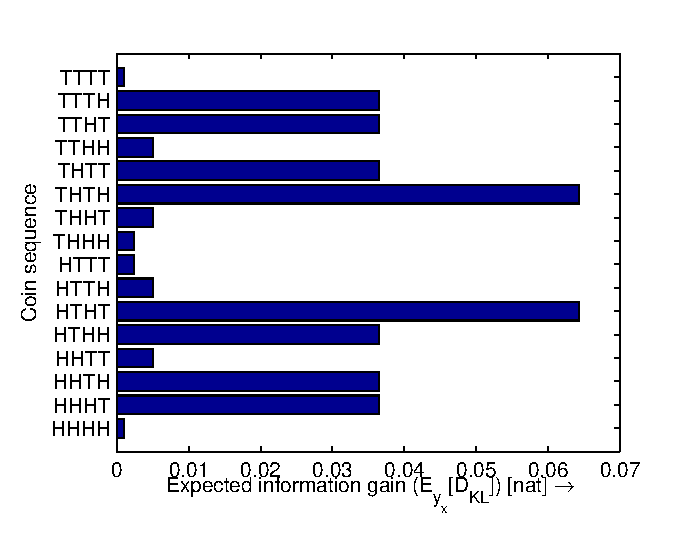
\includegraphics[width=3in]{img/coin.eps}
\caption{The information gain for all four flip coin sequences experiment prompts.}
\label{fig:coin}
\end{figure}

The most informative experiment prompts are the symmetric pair of coin sequences `HTHT' and `THTH'. 
In this case, the weighted coin observes two heads and two tails and infers that the bias should be centered around 0.5; this model does not favor either heads or tails as the next coin flip. 
In comparison, the Markov coin model infers that the flip sequence is alternating, and thus strongly favors the heads as the next coin flip in the first sequence, and tails for the second sequence. 
%By exploiting this difference in predictions, one can easily determine the underlying model from the response.

Following the same logic, the least informative experiment prompts are the symmetric pair of coin sequences `HHHH' and `TTTT'. 
For \lstinline{HHHH}, the bias coin observes all heads and infers that the coin is heavily biased towards a heads outcome for the next coin. 
The Markov coin model infers that the flip sequence is unlikely to transition, and thus, also strongly favors a heads outcome for the next coin. 
Although each model has differing rationales for their predictions, they share the same prediction which makes it very difficult to determine the underlying model from an response.

Optimal experiment design can be used to gain general insights about both the experiment space and the candidate models. For example, the information gain is symmetric with respect to heads and tails symbol inversion.  In the case of coin flips, it is intuitive why this is the case. When we move to more complicated experimental and modeling spaces, one can get a deeper understanding of the capabilities and limitations of the candidate models by observing the information gain of experiments.

\subsection{Experiments?}


\section{Case study 2: Category learning}

We now consider a more elaborate example in the domain of category learning. The ability to form concepts and abstract rules is an integral component of cognitive science as it establishes a foundation for naming objects and events, as well as discussing and interacting with them. Since few concepts are formally taught, the formation and progression of classifying observations and experience into categories must be a fundamental learning phenomenon. As such, models of classification learning has been an active area of research in cognitive science for decades~\cite{machery10:bbs}. 

 This case study builds on the classic experiment from Medin and Schaffer~\cite{medin78:pr}, and illustrates how computational approaches to experiment design can often outperform human intuition. In particular, this case study demonstrates the efficacy of OED in psychology for discrete and non-ordinal experiment spaces, large combinatoric experiment spaces, and parametric model classes. 

\subsection{Models of Classification Learning}

In this case study, we consider two formal models of classification learning: the Context Theory model and the Independent Cue model, which were the two models originally compared by Medin and Schaffer. These models were selected since they are well-known computational models that are well-suited for comparison described in a classic paper on classification learning. Furthermore, the authors describe their experiment design process in detail to explain how it is capable of differentiating the two candidate models, making this scenario ideal for evaluating whether automated experiment design approaches can outperform expert intuition. 

Following the experimental setup of Medin and Schaffer, participants are provided with exemplars from two categories and prompted to classify a set of stimuli individually (described in further detail in Section~\ref{ss:ms_setup}). The space of classification learning models under consideration is $\mathcal{M} \in \{m_{ct}, m_{ic}\}$, where $m_{ct}$ and $m_{ic}$ correspond to the Context Theory model and the Independent Cue model, respectively. The space of experimental prompts, $\mathcal{X}$, is the joint set of all possible training exemplars and probe stimuli, and the space of responses, $\mathcal{Y}$, is set the classifications of all the probe stimuli.

\subsubsection{Notation}

Before introducing the classification models, it is useful to discuss the notation for representing stimuli. The stimuli to be classified is represented as a composition of binary properties of four cue dimensions: color (red or blue), form (triangle or circle), size (large or small), and number (one or two). Each stimuli can be described using a binary code with `0' and `1' representing one of the properties, respectively. For example, using the dimension ordering of color, form, size and number, the notation `1001' might refer to a single small red circle, while `0110' would refer to a stimulus comprised of two large blue triangles. This binary code makes it easy to compare the similarity of stimuli: `1111' and `1101' differ only in size, while `0101' and `1101' differ only in color. 

\subsubsection{Context Theory Model}

The first classification model is the Context Theory model, which is built upon seven explicitly stated assumptions~\cite{medin78:pr}. For the purposes of computational experiment design, the two most relevant cognitive assumptions are that category judgements are based on the retrieval of exemplar information and that the overall similarity of two stimuli are comprised of multiplicative combinations between the similarity of retrieval cues. These assumptions are formalized as a statistical model that uses a sum of product computation to determine the probability a stimulus will be associated with a given category.

Formally, let the variables $x_A$ and $x_B$ represent the sets of stimuli that correspond to exemplars in category A and category B, respectively. Furthermore, let the variable $x_s$ represent the set of stimuli that correspond to the probe stimuli, which is mutually exclusive with the category exemplars. Let the random variable $Y \in \{A,B\}^{|x_s|}$ represent the probability that each probe stimuli is classified to belong in a corresponding category. Let the variable $c_i$ represent the $i$th cue dimension and let the variable $w_i$ represent the corresponding model weighting parameter. The probability that the Context Theory model will classify the $k$th probe stimuli, $x_{sk}$, in the category $y_k$ is then defined as:
\begin{align}
    p(y_k | x_{sk}, x_A, x_B, w_1, \dots, w_d) &= \frac{\sum\limits_{x_j \in y_1} \prod\limits_{i=1}^d f_{ct}(x_{ski}, x_{ji}, w_i)}{\sum\limits_{c \in \{A,B\}}\sum\limits_{x_j \in c} \prod\limits_{i=1}^d f_{ct}(x_{ski}, x_{ji}, w_i)}, \label{eq:ct_base}
\end{align}
where $d$ is the size of the cue dimensions, and $f_{ct}$ is the similarity measure:
\begin{align}
    f_{ct}(x_{ski}, x_{ji}, w_i) = 
        \begin{dcases}
            1  , & \text{if } x_{ski} = x_{ji}\\
            w_i, & \text{otherwise}
        \end{dcases}.
\end{align}

\begin{figure}[h]
\hspace{1cm}
\begin{tabular}{ccccccccccc}
\multicolumn{5}{c}{Category A} & \hspace{1cm} & \multicolumn{5}{c}{Category B} \\
Stimulus & \multicolumn{4}{c}{Pattern} & & Stimulus & \multicolumn{4}{c}{Pattern} \\
  & $c_1$ & $c_2$ & $c_3$ & $c_4$ & & & $c_1$ & $c_2$ & $c_3$ & $c_4$  \\ \cline{2-5} \cline{8-11}
$s_1$ & 1 & 0 & 1 & 1 & & $s_4$ & 0 & 0 & 0 & 0 \\
$s_2$ & 1 & 1 & 1 & 0 & & $s_5$ & 0 & 0 & 1 & 1 \\
$s_3$ & 1 & 1 & 1 & 1 & & $s_6$ & 1 & 1 & 0 & 0 
\end{tabular}
\vspace{1cm}
\newline
\begin{tabular}{ccccc}
\multicolumn{5}{c}{Probe Stimuli} \\
Stimulus & \multicolumn{4}{c}{Pattern} \\
  & $c_1$ & $c_2$ & $c_3$ & $c_4$ \\ \cline{2-5} 
$s_7$ & 1 & 0 & 1 & 0 
\end{tabular}
\centering
\caption{An example set of stimuli for Category A, Category B, and probe stimuli.}
\label{fig:cat_example}
\end{figure}

To clarify the computation of Eq.~\ref{eq:ct_base}, consider the example shown in Fig.~\ref{fig:cat_example}. Using the provided set of stimuli, the probability that the probe stimulus will be classified in Category A is: 
\begin{align}
    p(A | x_s, x_A, x_B, w_1, \dots, w_d) 
        &= \frac{(1\!\cdot\!1\!\cdot\!1\!\cdot\!w_4) + (1\!\cdot\!w_2\!\cdot\!1\!\cdot\!1) + (1\!\cdot\!w_2\!\cdot\!1\!\cdot\!w_4)}{ \splitfrac{(1\!\cdot\!1\!\cdot\!1\!\cdot\!w_4) + (1\!\cdot\!w_2\!\cdot\!1\!\cdot\!1) + (1\!\cdot\!w_2 \cdot\!1\!\cdot\!w_4)}{+ (w_1\!\cdot\!1\!\cdot\!w_3\!\cdot\!1) + (w_1\!\cdot\!1\!\cdot\!1\!\cdot\!w_4) + (1\!\cdot w_2\!\cdot\!w_3\!\cdot\!1)}} \notag \\
        &= \frac{w_4 + w_2 + w_2w_4}{w_4 + w_2 + w_2w_4 + w_1w_3 + w_1w_4 + w_2w_3}. 
\end{align}
If all four parameters were equal to 0.3, then the probe stimulus $s_7$ should be classified in Category A with a probability of 0.72. 

As the model parameters are not a part of the experiment design, they must be marginalized out by using a prior distribution over the model parameter, $p(w_i)$:
\begin{align}
    p(y_k | x_{sk}, x_A, x_B) &=  p(y|x_{sk}, x_A, x_B ,w_1, \dots, w_n) p(w_1) \dots p(w_d),
\end{align}
which leverages the property that each model parameter, $w_i$, is independent.

Finally, the probability of classifying a set of probe stimuli for the Context Theory model is computed using: 
\begin{align}
    p(y_{1,\{x_{s1}, x_A, x_B\}}, \dots, y_{n,\{x_{sn}, x_A, x_B\}} | m_{ct}) &=  \prod\limits_{k=1}^{|x_s|} p(y_k|x_{sk}, x_A, x_B).
\end{align}

The WebPPL program for the Context Theory model is shown in Fig.~\ref{fig:webppl_ct}. TODO: The program begins with defining general utility code (lines~\ref{ln:wbc_help_s}-\ref{ln:wbc_help_e}): a helper function for sampling from a categorical distribution and the manual definition of the model parameter prior distributions, which are assumed to be uninformative prior or the uniform distribution. Talk about prior distributions. Talk briefly about the model. 


\subsubsection{Independent Cue Model}
The second classification model is the Independent Cue model, which assumes that the information entering category judgments can be derived from an additive combindation of the information from the component cue dimensions. Prototype, average distance and versions of cue validity and frequency models fall under this domain. This is a prototype model that classifies probe items by comparing similarities with a representative prototype of the category




Formally, let the variables $x_A$ and $x_B$ represent the sets of stimuli that correspond to exemplars in category A and category B, respectively. Furthermore, let the variable $x_s$ represent the set of stimuli that correspond to the probe stimuli, which is mutually exclusive with the category exemplars. Let the random variable $Y \in \{A,B\}^{|x_s|}$ represent the probability that each probe stimuli is classified to belong in a corresponding category. Let the variable $c_i$ represent the $i$th cue dimension and let the variable $w_i$ represent the corresponding model weighting parameter. The probability that the Context Theory model will classify the $k$th probe stimuli, $x_{sk}$, in the category $y_k$ is then defined as:

This is formalized as a rank-ordering model that uses an additive computation to determine the relative association with a given category

The first thing we need to consider is the information value and wthe associated weighting factor. When a pattern is presented to be classified at some point, the value associated witht eh color dimension will be sampled. If red is sampled, then the information would be positive since red is more closely associated with category A than B. If blue were sampled, then the information would be negative. This all depends on how informative each cue dimension is. Since this is all weighted anyways, we only really care about the relative information of each cue dimension, which we compute by computing the difference of positive examples over the total number of examples. The formulation is as follows:

\begin{align}
    f_{ic,A}(x_s, x_A, x_B, i) &= 
        \begin{dcases}
            \frac{\sum\limits_{x_a \in x_A} x_{ai} - \sum\limits_{x_b \in x_B} x_{bi}} {\sum\limits_{x_a \in x_A} x_{ai} + \sum\limits_{x_b \in x_B} x_{bi}}, & \text{if } x_{si} = 1 \\
            \frac{\sum\limits_{x_a \in x_A} (1-x_{ai}) - \sum\limits_{x_b \in x_B} (1-x_{bi})} {\sum\limits_{x_a \in x_A} (1-x_{ji}) + \sum\limits_{x_b \in x_B} (1-x_{bi})}, & \text{otherwise } 
        \end{dcases}
\end{align}

The good part of this formulation is that relective, where the information that a stimula is associated with catefory a is more likely to be associated with category b is simply the negative of each other:

\begin{align}
f_{ic,B}(x_s, x_A, x_B, i) = -f_{ic,A}(x_s, x_A, x_B, i)
\end{align}

Formulation into evidence? This gives a rank-ordering model.

To convert this rank-ordering model into a statistical one, we use a log-linear transformation to convert the relative associations into probabilities. Something about bayesian interpretation?

\begin{align}
    P(Y=A| x_s, x_A, x_B, w_0, w_1, \dots, w_d, \alpha) &= 
        \begin{dcases}
            \frac{1}{1 + e^{-\alpha \left(w_0 + \sum \limits_{i=1}^d w_i f_{ic,A}(y, x, i)\right)}}, & \text{if } x_s \in \{x_A \cup x_B\}\\
            \frac{1}{1 + e^{-\alpha \left(\sum \limits_{i=1}^d w_i f_{ic,A}(y, x, i)\right)}}, & \text{otherwise }
        \end{dcases}
\end{align}

$P(Y=B| x_s, x_A, x_B, w_0, w_1, \dots, w_d, \alpha) = 1- P(Y=A| x_s, x_A, x_B, w_0, w_1, \dots, w_d, \alpha)$, which arises from the property that $1-\frac{1}{1+e^{-x}} = \frac{1}{1+e^x}$, and $f_{ic,B}(x_s, x_A, x_B, i) = -f_{ic,A}(x_s, x_A, x_B, i)$.

Example.

\begin{align}
    p(y | x_s, x_A, x_B) &=  
        \begin{dcases}
            p(y|x_s, x_A, x_B, w_0, w_1, \dots, w_d, \alpha) p(w_0) p(w_1) \dots p(w_d) p(\alpha), & \text{if } x_s \in \{x_a \cup x_b\}\\
            p(y|x_s, x_A, x_B, w_1, \dots, w_d, \alpha) p(w_1) \dots p(w_d) p(\alpha), & \text{otherwise}
        \end{dcases}
\end{align}
since each $w_i$ is independent.

For a collection of stimuli, 
\begin{align}
    p(y_{1,\{x_{s1}, x_A, x_B\}}, \dots, y_{n,\{x_{sn}, x_A, x_B\}} | m_{ic}) &=  \prod\limits_{k=1}^n p(y_k|x_{sk}, x_A, x_B) 
\end{align}

code?

\subsection{Optimal Experiment Design}
With meticulous forethought, MS designed an experiment to disambiguate these two candidate models and then analyzed participant's performance on using this prompt. The prompt is shown in Fig. Explain the logic in their prompt.

Although MS provide sound arguments for their experiment design, does their experiment provide the optimal amount of information for disambiguating their competing models?

Constrained to the same MS experiment space, we exhaustively evaluated the 933 valid and unique experiments in terms of expected information gain

In particular, this case study demonstrates the efficacy of OED in psychology for discrete and non-ordinal experiment spaces, large combinatoric experiment spaces, and parametric model classes. 

\subsection{Results and Discussion}

MS is a suboptimal experiment that ranks in the 30$^\text{th}$ percentile with respect to expected information gain (Fig.~\ref{fig:dist})
\begin{figure}[h!]
\centering
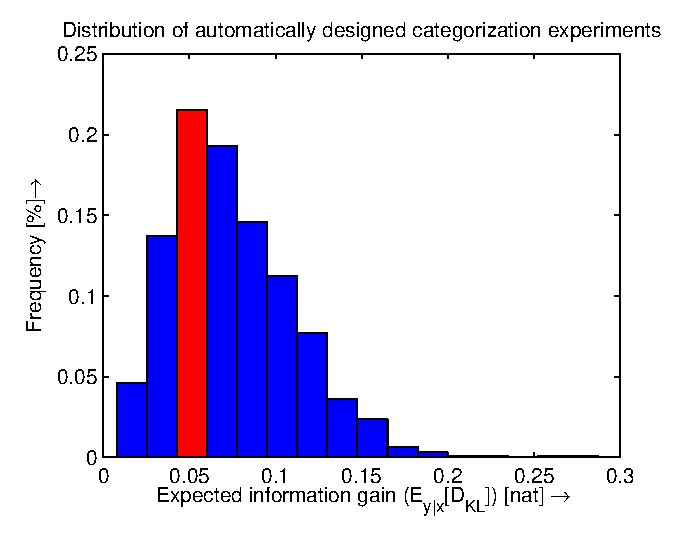
\includegraphics[width=3.2in]{img/dist.eps}
\caption{The distribution of optimal experiments with the MS bin highlighted in red.}
\label{fig:dist}
\end{figure}

The MS uses a qualitative swap in ranking for two stimuli to disambiguate the models. However, this prediction has a relatively small magnitude and comes at the expense of little information gain from the remaining stimuli. The optimal experiment is better able to quantitatively disambiguate the models by maximizing the information from all the stimuli simultaneously

The MS and optimal experiments were used to gather data from human participants on Mechanical Turk

The empirical results verify the OED predictions that the optimal experiment better disambiguates the two models (Fig.~\ref{fig:empirical})
\begin{figure}[h!]
\centering
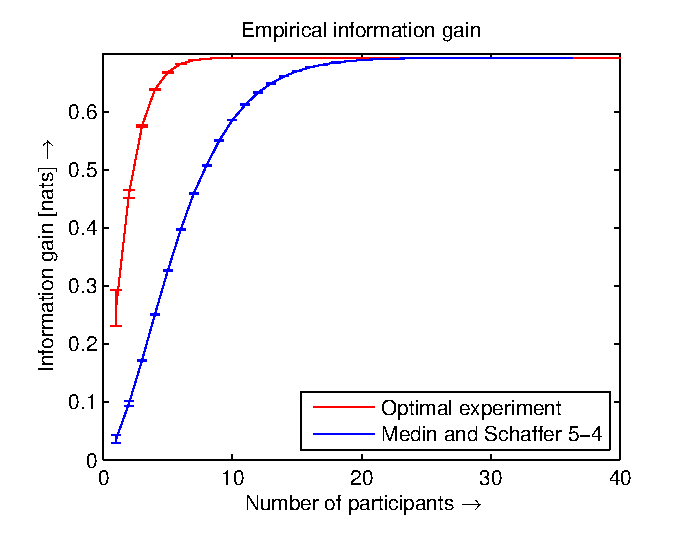
\includegraphics[width=3.2in]{img/empirical.eps}
\caption{Empirical information gain from $(n=40)$ Mechanical Turk participants. Error bars indicate standard error.}
\label{fig:empirical}
\end{figure}


\section{Relationship to previous work}
\section{Discussion}

The purpose of \red{our(?)} OED approach is to quantify the ability of an experiment to differentiate competing computational models. Our approach leverages Bayesian inference to reason about which model best describes a given phenomenon. By using the models' predictions to compute the likelihood of observing a particular response to an experiment, this approach provides a rational method for updating the change in belief about model uncertainty when such responses are observed. This change in belief is then quantified using information theoretic measures, and by maximizing these measures, OED allows one to find experiments that should maximally change the uncertainty of the beliefs in our models.


In this paper, we focus our analysis on the OED criteria of expected KL divergence and its properties, as opposed to the argument of the maximum component of the expression. \ndg{?} The reason is that Eq.~\ref{eq:oed} can rarely be solved analytically and solving it numerically is often a daunting task. To illustrate the advantages of our OED approach, we will be exhaustively evaluating the expected KL divergence for the entire  space of experimental prompts. This allows us to obtain a comprehensive analysis of the entire design space, and the challenge of selecting the optimal experiment is reduced to a simple sorting task. For large design spaces where exhaustive search is intractable, numerical optimization approaches, such as Sequential Monte Carlo searches (REF) or Bayesian optimization (REF), are viable options.  \ndg{move this to dicussion?}



\lou{say some stuff about OED for non-psych experiments}

%\bibliographystyle{ieeetr}
%\bibliography{oed_nips_2016}

\end{document}
